\documentclass{article}
\usepackage[T1]{fontenc}
\usepackage{setspace}
\usepackage[table]{xcolor}
\usepackage[margin=1in]{geometry}
\usepackage{tabularx}
\usepackage{enumitem}
\usepackage{outlines}
\usepackage{hyperref,verbatim}
\setcounter{tocdepth}{3}
\setcounter{secnumdepth}{0}
\usepackage{array}
\usepackage{babel}
\usepackage{caption}
\usepackage{graphicx}
\usepackage{svg}
\usepackage{subfigure, wrapfig}
\usepackage{amssymb, amsmath}
\usepackage{tikz,mathtools,amssymb}
\usetikzlibrary{shapes,arrows,positioning,calc}
\usetikzlibrary{arrows.meta} % For arrow tips
\usepackage{epsdice}
\usepackage[resetlabels,labeled]{multibib}

\setlist{nolistsep}

\definecolor{blue}{HTML}{008ED7}
\definecolor{lightBlue}{HTML}{e5f7ff}
\newcommand{\n}{\cellcolor{green!10} not capable}
\newcommand{\y}{\cellcolor{purple!10} capable}

\renewcommand{\familydefault}{\sfdefault}
\renewcommand{\arraystretch}{1.5}

\title{Katzenpost Threat Model}
\author{David Stainton \and Eva Infeld}

\newcites{C}{Selected sources on adversaries}
\newcites{A}{Selected sources on attacks}

\begin{document}

\maketitle
\begin{abstract}
\noindent We describe the threat model of the Katzenpost mix network transport protocol and discuss the threat models for additional protocol layers. We start with an overview of the capabilities of our adversaries, and list the commonly considered attacks these adversaries are capable of. We then summarise the countermeasures employed by Katzenpost against these attacks. Finally, we point out certain attacks Katzenpost doesn't yet mitigate, and discuss future attack countermeasures.
\end{abstract}

\small
\tableofcontents
\normalsize

\section{The purpose and structure of this document}

This threat model document is unique in the privacy technology landscape for its detailed treatment of realistic adversary capabilities. It is not a description of a superficial, theoretical system, but rather of complex, real-life software that is being interrogated and constantly re-designed to provide the best possible security. We examine it from the point of view of both theoretical design, networking choices and practical pitfalls. 

And still, it is not and will likely never be comprehensive. Various attacks and countermeasure strategies will be added to this document in the future, as it keeps evolving. However, we feel that it already provides a valuable, systematic view of the challenges faced by mixnet technology.

There exists a rich body of academic work analyzing how one might disrupt the functioning of a Mixnet or circumvent its security and privacy guarantees. We have endeavored to compile these decades research and summarized these attacks in the table on page 3. The table on page 4 focuses on networking security threats that are specific to Katzenpost protocol choices.

We then delve into the countermeasures employed by Katzenpost and discuss their efficacy. A special care is taken to discuss the details of post-quantum cryptographic primitives that we have introduced in several places of the design.


\section{Introducing the adversary}

It is no longer controversial to say that in the modern world, we face incredibly powerful surveillance adversaries. These could be state, corporate or criminal actors, vying for our information to use as means of making profit, manipulating us and others, gaining leverage, strengthening their authority, or as means of persecution. In many contexts, we have little hope for non-technical solutions due to lack of sufficiently powerful pressure in favor of privacy.

And so in a quest for technical solutions, we need equally powerful tools. In the case of communication tools, the Internet's bread and butter, we would like to allow users to interact and exchange information with reasonable expectation of both the content and metadata of their communication, and personal information such as a user's social graph, being protected from such adversaries. Therefore, we consider an adversary capable of the following:
\begin{itemize}
\item The adversary can see the connections of the entire global internet and is capable of intricate statistical analysis of gathered data.
\item The adversary can disable parts of the network.
\item The adversary can plant or take over some devices in the network to inject malicious code and manipulate the functioning of the network or to gain access to the information available to them. The takeover could happen by technical means or by exercising force outside of the network.
\item The adversary has very large (but not infinite) computational resources, and is capable of cryptanalysis on par with frontier research.
\item The adversary has access to a quantum computer, or will have access to a quantum computer in the near future.
\item The adversary can supplement collected data with rich context of already gathered data on all users from other sources.
\end{itemize}

If we hope for our work to be relevant in the modern world, we can no longer settle for weak threat models. That is the bar we set for ourselves at Katzenpost.

\pagebreak

\section{Katzenpost mixnet threat model summary}

Firstly, assumptions about the user:\\

\begin{enumerate}
\item The user acts reasonably and in good faith.
\item The user obtains an authentic copy of the Katzenpost client and the mixnet client configuration file.
\end{enumerate}
\vspace*{5px}

\noindent Secondly, assumptions about the user's computer:\\

\begin{enumerate}
\item The computer operates correctly and is not compromised by malware.
\end{enumerate}
\vspace*{5px}

\noindent Thirdly, assumptions about the mixnet:\\

\begin{enumerate}
    \item The mixnet only provides internal services and does not have any "exit nodes" or anything that resembles a proxy service or VPN.
    \item All mixnet protocols are protocols which do not force interaction.
    \item All mixnet protocols are low bandwidth and latency tolerant.
\end{enumerate}

\noindent Finally, assumptions about the world:\\

The three core protocols of Katzenpost are configured to use modern cryptographic primitives which are valid and considered impossible to break, for example:

\begin{itemize}
  \item PKI Signature Scheme using Edd25519-Sphincs+
  \item NIKE Sphinx using X25519
  \item PQ Noise with pqXX pattern using Xwing
\end{itemize}
\vspace*{5px}

\noindent What the user's Gateway can achieve keeping in mind that
typically a fair sized mixnet will have more than one gateway node:\\

\begin{itemize}
    \item A Gateway node learns when a given client is online.
    \item A Gateway node learns the client's IP address.
    \item A Gateway node learns how many messages the client sends and receives.
    \item A Gateway node does NOT learn the sent message destinations or the received message origins.
    \item A Gateway node does NOT learn if a given sent or received message is a decoy or not.
    \item A Gateway node can drop or correupt any sent or received message.
    \item A Gateway node can spam a user with invalid messages.
    \item A Gateway node can duplicate old messages. However duplicate outbound messages will be dropped by the first hop as per Sphinx packet deduplication cache.
\end{itemize}
\vspace*{5px}

\noindent What a sufficiently global, passive adversary can achieve:\\

\begin{itemize}
    \item A GPA can learn who is using the mixnet and where their Gateway nodes are located.
\end{itemize}
\vspace*{5px}

What a local network attacker can achieve:\\

\begin{itemize}
    \item A local network can observe when a user is using Katzenpost.
    \item A local network can block Katzenpost.
\end{itemize}
\vspace*{5px}

\noindent What a compromise of the user's computer can achieve:\\

After an endpoint device is compromised, an attacker can impersonate that user, receiving and sending messages. The attacker does NOT learn the communication correspondent network locations.
\vspace*{5px}

What a Service Node can achieve:\\

A Service Node on the mix network does not know from whence it's service request message came.
Therefore in general, absent some clever attack, the Service Nodes learn nothing about the clients
that interact with them.
\vspace*{10px}

What a contact can achieve:\\
\begin{itemize}
    \item A contact can spam a user with messages.
    \item A contact can, to some extent, prove to a third-party that a message came from a user
    \item A contact can retain messages from a user, forever.
\end{itemize}
\vspace*{10px}

What a random person on the Internet can achieve:\\

A random person can attempt to DoS the mix network or a specific service on the mixnet.


\pagebreak
\section{A summary of theoretical security concerns in a Mixnet}

\small
\begin{center}
\fontfamily{cmss}\selectfont
\begin{tabularx}{\textwidth}[t]{|m{0.15\textwidth}| m{0.38\textwidth}| m{0.39\textwidth}| }
\arrayrulecolor{blue}\hline 
\rowcolor{lightBlue} 
\textbf{\textcolor{blue}{Mixnet \linebreak attack type}} & \textbf{\textcolor{blue}{Attack description}} & \textbf{\textcolor{blue}{Necessary adversary capabilities}} \\

\hline Intersection, Statistical Disclosure Attacks & Over time, adversary can glean statistical information that makes the probability distribution of who Alice is communicating with non-uniform. Law of Large Numbers implies the anonymity set tends to the set of clients with identical probability in the long run to the actual recipient. & The adversary must typically be able to see messages entering and leaving the network. This is customarily treated as a PGA, despite only requiring a view of the network's perimeter. The adversary must be able to distinguish messages from dummy traffic, or  observe when users are active.
\\
\hline $n-1$ Attack & The adversary causes the mix to contain only messages sent by the adversary, except one.  In the context of continuous time mixing such as with the Poisson mix, this means that the adversary drops or delays other messages until the mix is empty before the target message enters the mix. The adversary sees the target message exit the mix to its next destination. & The adversary must compromise routers which are upstream from a target mix node so as to be able to block incoming messages, send messages, as well as be able to tell when a target message passes through them.\\

\hline Epistemic Attack & The fact that a client is issued only a subset of the mix nodes' directory and encryption keys can leak information to the adversary.\medskip

&  The adversary has knowledge of the target client's view of the network which distinguishes them among clients. This could happen via a zero day or a design flaw such as not implementing PIR for discovery. \\
\hline Denial of Service Attack & The adversary is able to disrupt the functioning of the service, often by overwhelming its resources. & The adversary has sufficient network and computational resources to overwhelm the network. \\
\hline Sybil Attack & The adversary plants a large number of malicious nodes, and is therefore able to glean partial or complete information to follow a message through the mix and disrupt the network. & The adversary has sufficient resources to take over the network, and the network's design allows for the creation of a large number of malicious nodes.\\
\hline Compulsion Attack & The adversary compels enough honest node operators to disclose information to follow a message through the mix network . & The adversary has the necessary force to compel a sufficient number of honest actors to do the adversary's bidding. \\
\hline Timing Attack & An active adversary manipulates the timing of the packets passing through compromised routers, or passive adversary exploits timing information that is leaked despite padding. & 
The passive attack could happen via a zero day or design flaw. The efficacy of the active attack needs to be analyzed with respect to the specific design.\smallskip

\\
\hline Cryptographic Attacks & The adversary is able to forge a signature, generate a second hash preimage, decrypt cyphertext or do other damage assumed to be prevented by the use of cryptography. & The adversary can break the security of one or more cryptographic primitives through a cryptographic zero day or sufficient computational resources, or exploit a flaw in their implementation.  \\


\hline Endpoint Security Attacks & The adversary breaches the security of a user's device via an attack not directly related to the mixnet. & The adversary is able to exploit a technical flaw in the user's device or compel the user to grant him access.\\

\hline Predecessor Attack & The adversary compromises at least one  mix node in each routing topology layer. Eventually a client will randomly select a bad route where every mix node in the route is compromised. & The adversary must have the capability to operate or compromise mix nodes, at least one in each routing topology layer. See countermeasure section for more details.
\\


\arrayrulecolor{blue}
\hline
\end{tabularx}
\end{center}
\pagebreak

\normalsize

\section{Networking security concerns in Katzenpost}
\begin{center}
\fontfamily{cmss}\selectfont
\begin{tabularx}{\textwidth}[t]{|m{0.15\textwidth}| m{0.38\textwidth}| m{0.39\textwidth}| }
\arrayrulecolor{blue}\hline 
\rowcolor{lightBlue} 
\textbf{\textcolor{blue}{Mixnet \linebreak attack type}} & \textbf{\textcolor{blue}{Attack description}} & \textbf{\textcolor{blue}{Necessary adversary capabilities}} \\

\hline Tagging Attack & The adversary exploits some kind of cryptographic malleability property of the Sphinx packet format in order to violate the privacy notions of the mix network. 
& The adversary must be able to witness the Sphinx payload decryption to determine if it was tagged or not. This means compromising a Provider for forward packets and compromising a client's endpoint device for SURB replies.\\

\hline Replay Confirmation Attack & If a Sphinx packet is able to be replayed then the adversary may send the packet many times concurrently in order to observe the traffic burst in another part of the network.  & The mix nodes maintain Sphinx replay caches in order to prevent replays; the attack is therefore only possible if there is a replay cache malfunction. \\

\hline SURB Confirmation Attack & If a client sends many SURBs\footnote{Sphinx Single Use Reply Block is essentialy a one-time use privacy preserving delivery token} to another entity on the network, that entity may choose to send out ALL the SURBs at once in order to observe the traffic burst in another part of the network. & The adversary is a global passive observer of the network and participant in the network; additionally the adversary must be in possession of multiple SURBs created by another entity on the network. \\

\hline ARQ Confirmation Attack & The adversary's goal is to find a specific ARQ\footnote{Automatic Repeat reQuest is a category network error correction strategies that uses retransmissions and acknowledgement packets} client who is currently interacting on the network by causing targeted outages of entry Providers after the target service receives a protocol message. To start, half of the entry Providers are allowed to receive messages. If the adversary observes a retransmission then it confirms the client is in the group of entry Providers that we blocked messages to. The adversary continues the binary search and finds the client's entry Provider in log(n) time. & The adversary must have access to a target mixnet service so as to distinguish a message transmission versus a retransmission. The adversary must also be able block messages from going to specific mixnet nodes, in this example, entry Providers. \\



\arrayrulecolor{blue}
\hline
\end{tabularx}
\end{center}
\pagebreak


\section{Attack Countermeasures}

Here we describe the attack countermeasures currently used by the Katzenpost mix network software design.

\subsection{Intersection Attacks}

\paragraph{Attack description:}
Intersection attacks, also known as long term statistical disclosure attacks have two basic categories:\\
\begin{enumerate}
    \item The Adversary learns to whom Alice sends messages.
    \item The Adversary learns who sends Alice messages.
\end{enumerate}

\paragraph{}Statistical disclosure attacks work to some extent on all
anonymous communication networks. The Katzenpost client and Katzen
messaging protocol is designed to provide partial defense against long-term
intersection attacks as well as sufficient defence against short-term timing
correlation attacks.

The simplest form of this attack assumes a global passive adversary who watches Alice's interactions
with the mix network. Whenever Alice sends a message, a set of potential recipients are noted by observing
which clients receive a message shortly after Alice sends her message. After many
hours, days or weeks of noting these sets of potential recipients, an intersection among these sets may reveal
the set of recipients Alice sends messages to.

The classical mix network literature has described intersection
attacks in terms of a mix network where a passive network
observer can watch individual clients receive messages. This
assumption can be otherwise stated that the adversary observes
all the inputs and outputs of the mix network and thus
receives a high granularity of statistical information. 

\paragraph{countermeasure}

Katzenpost and the Katzen messaging protocol are designed to provide partial defense against intersection attacks.
Complete defense is not practical because user behavior is often repetitive and they cannot stay connected to the mixnet forever.
Attack success depends largely on the adversary's ability to predict user behavior.
If user's behavior is overly repetitive this may lead to the success of such attacks.

Although the Katzenpost continuous time mixing strategy provides defense against short term timing correlation attacks,
additional defense mechanisms are required to defend against longer term attacks:\\

\begin{enumerate}
    \item async message queueing and retrieval at the network edge
    \item traffic padded message retrieval
    \item loop decoy traffic
    \item uniform traffic patterns (all sent messages result in a SURB reply)
\end{enumerate}

\paragraph{}The Katzenpost chat protocol known as Katzen, uses an additional network route
to provide another indirection to protect the network location of clients. In other words,
while Katzen clients connect to the mixnet using a randomly selected entry Provider, they
retrieve messages from a different Provider mix node on the network; message retrieval is done
by means of a Sphinx SURB, single use reply block which is sent to the messaging queue service
so that a reply containing a message payload can be sent back to the client, anonymously.
All sent messages result in a SURB reply being sent back to the client.

Katzenpost clients periodically send loop decoy messages; these Sphinx packets are sent to a randomly
selected Provider whose echo service sends the client's packet payload back to the client via
the attached SURB. However, loop decoy messages are only distinguishable from normal messages to
the client that receives them. Passive network observers will not be able to tell the difference.
These decoy loops are uniformly distributed among all of the Providers (AKA service/exit mix nodes).

Whenever clients retrieve messages from their locally connected entry Provider, they do so using a
traffic padded protocol that either sends them 0 or 1 message where both outcomes are indistinguishable from the
perspective of a passive network observer.


\pagebreak

\subsection{$n-1$ Attacks}

\paragraph{attack description:} An $n-1$ attack is a multi stage attack where the adversary observes a target message enter the mixnet
and must perform the attack in order to follow the message to the next hop. The $n-1$ attack is performed repeatedly for each hop in the route
in order to discover the final destination.

Although the adversary could simply compromise each mix node in the route starting with the first hop, that is the compulsion attack category
and is a distinct attack category from the $n-1$ attack category. The $n-1$ attack is performed by the adversary compromising upstream routers so that they have the capability
of watching messages enter the target mix, blocking any of those messages if they choose to, and sending messages of their own into the target mix node.
By using these capabilities the adversary is able to manipulate mix nodes so that they only contain the target message and messages sent by the adversary.

For a good introduction to $n-1$ attacks, please see \citeA{n-1}. In the context of continuous time mixing
strategies like "Stop and Go" \citeA{stopandgo} and Poisson \citeA{loopix}, the $n-1$ attack is performed by the adversary blocking or delaying
(although delaying obviously wouldn't work for Stop and Go) incoming messages ahead of time
so that they are reasonably certain the mix is empty before the target message enters the mix.

When the target message enters the empty mix, it is artificially delayed by the mixing strategy and then routed to the next hop.
The adversary gets to observe where the message is going for it's next hop because they are reasonably sure that the message
exiting the mix, although it is bitwise unlinkable because of the cryptographic transformation, it must be the same message.

\paragraph{countermeasure}: Katzenpost currently does not have any countermeasures in place for $n-1$ attacks. See Future Countermeasures section below.

\subsection{Epistemic Attack: route fingerprinting}

\paragraph{attack description:} A route fingerprinting attack is when the adversary is able
to identify a client by the specific route being used.

\paragraph{countermeasure:} Katzenpost doesn't allow clients to have a partial view of the network. The directory authority system publishes the full network view to be cached by the edge nodes, Providers, so that clients can retrieve them.

\subsection{Denial of Service}

\paragraph{attack description:}Sending many packets into the mix network can cause the mix
nodes to become overwhelmed and begin dropping packets. The logical conclusion to this scenario
is that there is effectively a network outage until the adversary stops sending so much traffic.

\paragraph{countermeasure:} Rate limiting individual clients is the current countermeasure. However this only stops the DOS attack from being conducted by a single client entity. However the adversary could still DOS the network by using many clients to send packets.

\subsection{Sybil Attack}

\paragraph{attack description:} The adversary plants a large number of
malicious nodes, and is therefore able to glean partial or complete information to
follow a message through the mix network.

\paragraph{countermeasure:} We mitigate Sybil attacks by preventing mix nodes from automatically
joining the network. A prerequesite for joining the network is to have all the directory
authorities add the new mix node's connection information and public cryptographic key material to their configuration. Please see the Future Countermeasures section below for a discussion
of additional directory authority features including a reputation system.

\pagebreak

\subsection{Compulsion Attack}

\paragraph{attack description:} The adversary compels enough honest node
operators to disclose information to follow a message through the mix network.

\paragraph{countermeasure:} Our current countermeasure for the compulsion attack is
frequent mix key rotation, every 20 minutes. See Future Countermeasures section below.

\subsection{Timing Attacks}

\paragraph{attack description:} An active adversary manipulates the
timing of the packets passing through compromised routers, or passive adversary
exploits timing information that is leaked despite padding.

Currently, there are no known timing attacks against any Katzenpost protocols.
Timing correlation attacks are already covered in the intersection
attack category. And although all mix network protocols leak statistical information no matter
what countermeasures are used, we posit that this leaked statistical information isn't really
the same thing as traditional timing attacks against a cryptographic system. In fact, the mix
network is actively preventing timing attacks injecting latency into the system.

\paragraph{countermeasure:} No known timing attacks and therefore no countermeasure.

\subsection{Cryptographic Attacks}

\paragraph{attack description:} There are no known cryptographic attacks against Katzenpost
core protocols (sphinx, noise, dirauth). However we explore theoretical cryptographic attacks
in the Cryptographic Protocols section below.

\paragraph{countermeasure:} All core Katzenpost protocols make use of hybrid post quantum cryptographic constructions which in theory protect against active quantum adversaries.

\subsection{Endpoint Security Attacks}

\paragraph{attack description:} The adversary breaches the security of a
user’s device via an attack not directly related to the mixnet.

\paragraph{countermeasure:} There are no countermeasures provided by Katzenpost for endpoint security because it's considered an orthogonal concern.



\subsection{Tagging Attack}

\paragraph{attack description:} The Sphinx cryptographic packet format allows for a
one bit tagging attack under certain circumstances. The reason
for allowing the design to have this security defect is to allow for the
Single Use Reply Block. The Sphinx header is MAC’ed but
the packet body is not. Instead, the body is encrypted with a
wide-block cipher (an SPRP). This ensures that an expected
verification block in the beginning of the plaintext can be used to verify the
plaintext in the final decryption. If a bit in the payload ciphertext gets flipped then the
payload decryption will yield garbled results and the expected verification block will not be present. Therefore in order to make
use of this to perform a tagging attack, the adversary must
have access to the result of the payload decryption
as well as the ability to tag the packet some number of hops
earlier in the route. We call this a one bit tagging attack because it yield one bit of information: Either the verification block was destroyed or not.

In Katzenpost there are two ways to use Sphinx to send a payload. Forwards packets and SURB reply packets. Both of these Sphinx packet types are susceptible to a one bit tagging attack:

\paragraph{tagging attack against forward Sphinx packets:} Clients send forwards Sphinx packets
to mixnet services which reply via a SURB in the payload. Let's say an adversary "tags" a forward Sphinx packet sent by Alice. The adversary would have to compromise or collude with
the service Providers on the mixnet in order to witness the forward packet payload decryption
failure which indicates the tag.

\paragraph{tagging attack against SURB replay Sphinx packets:} If an adversary "tags" a SURB reply which a mixnet service sends to a client, then only the client will be able to witness the packet payload decryption failure. The adversary would have to compromise the client's endpoint device to witness this event (or to compromise the key materials allowing them to compute the failed payload decryption themselves).

\paragraph{countermeasure:} In the context of a forward Sphinx tagging attack on Katzenpost,
the adversary must compromise or collude with the destination service Provider. If that's
the case then attack allows the adversary to learn which Provider node and service the packets was destined for. Although this is valuable information in the context of the current Katzen protocol, see the Future Countermeasures section below for a discussion of how we plan to mitigate intersection attacks in the future because it also carries over to much greater defense
against this forward payload tagging attack.

\paragraph{countermeasure:} We could encode the last hop's Sphinx routing command, inside the Sphinx payload instead of the header.
This would provide short term plausible deniability in the sense that an adversary conducting a tagging attack would be destroying
the routing information so that they cannot know if the packet was a decoy or not.



\subsection{Replay Confirmation Attack}

\paragraph{attack description:}
If a Sphinx packet were allowed to be replayed then the adversary may send the packet
many times concurrently in order to observe the traffic burst in another section of the
network.

\paragraph{countermeasure:} Katzenpost mix nodes maintain a relay cache which prevents Sphinx
packets from being replayed. This cache doesn't grow forever since it's only kept until the
end of the epoch which are currently only a 20 minute duration.

\subsection{SURB Confirmation Attack}

\paragraph{attack description:} If a client sends many SURBs to another entity on the network,
that entity may choose to send out ALL the SURBs at once in order to observe the traffic burst
in another part of the network. This works as an entry node discovery attack. 

Although currently, all Katzenpost protocols only send one SURB at a time, this attack still
applies if the adversary accumulates enough SURBs to form a visible traffic burst within the mix
network.

\paragraph{countermeasure:} No countermeasure. See Future Attack Countermeasure section below for the discussion of how to countermeasure this attack.

\subsection{ARQ Confirmation Attack}

\paragraph{attack description:} See above table entry for ARQ confirmation attack description.

\paragraph{countermeasure:} Currently, no countermeasure.

\subsection{Predecessor Attack}

\paragraph{attack description:} A bad route is defined as a route in which every node is compromised. The goal of such an attack is to link a given client with a specific destination or service on the destination node. This attack is also known as the Predecessor Attack and is detailed in \citeA{Wright:2004} with many variations for all the different types of anonymous communication networks. In the context of the Katzenpost mixnet, the Predecessor Attack is performed by the adversary compromising at least one node in each routing topology layer. Clients using the mixnet will eventually select a bad route.

\paragraph{countermeasure:} Fundamentally, we have two choices, either we have clients select a new route for each message sent or they select one route and use that for some time duration. In the former, every time a message is sent, the probability of selecting a bad route is increased. Whilst in the later, if a client selects a bad route they use it many times, but the probability of selecting a bad route is reduced.
\paragraph{}Yet another countermeasure is to design the mixnet protocols such that they use a new destination for each message using some kind of private deterministic permutation achieving a uniform distribution of message amongst the destination mixnet nodes and their message slots. We have chosen this last countermeasure  for Katzenpost and it will be detailed elsewhere in our literature.



\section{Future Countermeasures}

\subsection{Intersection Attacks}

\paragraph{}The new Katzen protocol is sometimes referred to as scatter queue.
Two communicating parties each exchange shared secrets which they use to determine
a new "mailbox" for each message. To be clear, this new protocol is an improved revision of the previous Katzen protocol where
each party chooses their own "mailbox" (queue Provider + queue ID); the difference here is
that instead of the two parties exchanging mailbox locations they exchange seeds which are
used to determinically generate mailbox locations for each message.

This new protocol still uses all four previously mentioned mechanisms to achieve countermeasure against intersection attacks
however the new "scatter queue" design drastically reduces the amount of metadata which can be collected by the operators
of the mailbox Provider mix nodes. We think this is a huge improvement to the threat model. But it would be great if we could
quantify the improvement using various anonymity metrics. Firstly, Shannon entropy seems applicable here because we can make
statements like "compared to the old protocol, scatter queue increases the entropy on Providers where malicious adversaries are
trying to correlate communicating party sets with messages arriving at specific mailboxes"; the new protocol makes this infeasible. 

Therefore we can say that the new Katzen messaging protocol mitigates or partially mitigates intersection attacks by means
of five mechanisms:\\

\begin{enumerate}
    \item async message queueing and retrieval at the network edge
    \item traffic padded message retrieval
    \item loop decoy traffic
    \item uniform traffic patterns (all sent messages result in a SURB reply)
    \item scatter queue
\end{enumerate}


\subsection{$n-1$ Attacks}

\paragraph{}Here we will attempt to describe a partial countermeasure wherein clients receive statistical
information from the network which is cryptographically signed by it's authors. Client use this data to decide
if there's an ongoing $n-1$ attack, if there is they disconnect from the network and try again later.

There are two sources of information about $n-1$ attacks:
\begin{enumerate}
    \item mix loops
    \item client loops
\end{enumerate}

\paragraph{Mix loops vs client loops} In theory mix loops can detect $n-1$ attacks in the context of a continuous time mix. Such an attack means
the adversary is dropping or delaying messages before they enter the mix. Therefore the mix originating loop decoy message
can function as a sort of heartbeat protocol that allow the mix to detect $n-1$ attacks. Obviously this mix loop decoy message
might get dropped by the network for various reasons that have nothing to do with an $n-1$ attack. The red green blue heartbeat mixnet paper (by george)
suggests the countermeasure of the individual mixes halting their routing of messages temporarily to thwart the $n-1$ attacks.
This would work but it would also probably create unnecessary outages. Instead we want a system that let's the client software
decide whether or not there is an ongoing $n-1$ attack. Clients can also detect such attacks with their own end to end loop decoy messages.
However we want the mixes to publish a signed certificate containing their mix loop statistics. Client will then download these mix loop statistics
from the providers and they will use those statistics along with their own client loop statistics to make decisions with regards to $n-1$ network status.

\vspace{1cm}

\textbf{TODO: add detailed description of client heuristics for deciding if there's an n-1 attack}



\pagebreak
\section{Core Cryptographic Protocols}

Katzenpost consists of three cryptographic protocols:\\

\begin{enumerate}
    \item PKI/Dirauth
    \item PQ Noise
    \item Sphinx
\end{enumerate}

\vspace{.5cm}

Katzenpost is an overlay network meaning that we aren't trying to replace IP (internet protocol).
Overlay means we build protocol layers that sit on top of existing Internet protocols.
Currently Katzenpost works over TCP/IP however in the future we plan to support QUIC/IP
as an optional transport that can be selected.

Katzenpost uses a PQ Noise based protocol known as the Katzenpost wire protocol, which
provides point to point transport security and authorization. The wire protocol enforces the mix network's topology
whereby the clients are only allowed to connect to gateway nodes, gateway nodes are only allowed to send packets to layer 1 mixes,
and layer 1 mixes are only allowed to send packets to layer 2 mixes etc.

Clients use the wire protocol to talk to gateway nodes to whom they send Sphinx packets. These Sphinx packets are encapsulated
within the encrypted PQ Noise messages and are therefore never exposed to passive network observers but if they were there
wouldn't in principle be any problem with that. This redundancy in security is often referred to as "defense in depth".

Besides within the mixnet itself, the wire protocol is also used to directly communicate with the directory authorities. Gateway nodes
retrieve the latest PKI document from the directory authorities and cache the document for the epoch duration so that clients can download the cached copy. This is a notably different use case because within the mixnet we should have the goal of padding all the wire protocol commands
to be the same size. Whereas when gateways nodes download the consensus they are likely receiving PKI documents which are perhaps many times bigger than our Sphinx packet size.

The PKI/Directory authority protocol stands apart from the rest because it's the
root of all authority within the mix network. The PKI provides the network participants with all the connection information and key materials they need to use the other two protocols, PQ Noise and Sphinx. It does so by publishing a PKI document every epoch (currently 20 minutes). This is necessary because the mixes destroy their old mix keys and create new mix keys for each new epoch thereby reducing the window for compulsion attacks to the epoch duration.

Both the PQ Noise based wire protocol AND our Sphinx protocols are considered to be transport protocols.
However the dirauth as the 3rd cryptographic protocol here refers to two aspects:

\vspace{.5cm}

\begin{enumerate}
    \item The client and mixnet interactions with the dirauth system; That is, the pki document itself it signed by a majority of the dirauth nodes AND the pki document contains the mix descriptor for each mix node in the network. The document also specifies the topology. Mix nodes and clients verify these cryptographic signatures.
    \item The dirauth's crash fault consensus cryptographic protocol for publishing new PKI documents every epoch.
\end{enumerate}


\pagebreak

\section{Katzenpost PKI / Directory Authority}

\begin{figure}[ht!]
\centering
\begin{tikzpicture}[every node/.style={draw, circle, minimum size=1cm}]
  % Define the style for the arrows with arrowheads at both ends
  \tikzset{arrowstyle/.style={<->,>={Latex[length=3mm]},<={Latex[length=3mm]}}}
  
  % Draw a pentagon with nodes placed at each corner
  \node[regular polygon, regular polygon sides=5, minimum size=5cm, draw=none] (p) {};
  
  % Draw the nodes at each vertex of the pentagon
  \foreach \i in {1,...,5} {
    \node (dirauth\i) at (p.corner \i) {dirauth\i};
  }

  % Connect the nodes with a full mesh of bidirectional arrows
  \foreach \i in {1,...,5} {
    \foreach \j in {\i,...,5} {
      \ifnum\i=\j\relax % Skip if both indices are the same
      \else
        \draw[arrowstyle] (dirauth\i) -- (dirauth\j);
      \fi
    }
  }
\end{tikzpicture}
\caption{The dirauth system has voting protocol rounds where each party exchanges votes with every other party.}
\end{figure}

\paragraph{}The public key infrastructure (PKI) protocol for Katzenpost, also known
as the Directory Authority or dirauth, is a decentralized system of nodes
which vote for each epoch's consensus document. If we used a BFT protocol instead
then the dirauth system would fail when 1/3 + 1 nodes failed. Therefore we can
say that our crash fault tolerant system is more robust because it will fail
when 1/2 + 1 nodes fail.

The Katzenpost PKI is the security root of the entire system because all clients
and network nodes will depend on the PKI to sign the consensus document for each epoch.
Currently epoch duration is every 20 minutes. The consensus document is essentially a view of
the network, it contains all the connection information and all the public cryptographic key materials
and signatures. Each mix node signs it's descriptor and uploads it to the dirauth nodes. Each dirauth
node signs the consensus. When clients or nodes download the consensus document they are able to verify
the dirauth node signatures on the document.

Currently we use a hybrid signature scheme consisting of the classical Ed25519 and the
post quantum stateless hash based signature scheme known as Sphincs+ with the parameters: `sphincs-shake-256f`

\pagebreak

\section{The Katzenpost Noise Protocol Layer}

Early versions of Katzenpost used the Noise cryptographic protocol framework; however we used
an HFS (hybrid forward secret) variation of XX handshake that used a post quantum KEM however it could not resist active quantum adversaries since the initial keys exchanged were classical ECDH public keys. Such constructions offer protections against current classical adversaries that record ciphertext transcripts in hopes of breaking them in the future with a cryptographically relevant quantum computer.

More recently, Katzenpost was made to use PQ Noise from the paper, entitled, Post Quantum Noise \citeA{pqnoise}.
The paper shows us that we can algebraically transform existing classical Noise handshake patterns into post quantum handshake 
patterns by replacing all usages of ECDH with KEM. In some of these transformations there's additional network interactions implied.

Our current, hybrid KEM uses our security preserving KEM combiner and the NIKE to KEM adapter
(ad hoc hashed el gamal construction). Our Noise protocol string is:

\vspace{.25cm}
Noise\_pqXX\_Kyber768X25519\_ChaChaPoly\_BLAKE2b
\vspace{.25cm}

Which means that our PQ Noise protocol uses the following cryptographic primitives:
\vspace{.5cm}


\begin{enumerate}
    \item Hybrid KEM: KEM Combiner + NIKE to KEM adapter + X25519 + Kyber768
    \item MAC: Blake2b
    \item AEAD: ChaChaPoly
\end{enumerate}

\vspace{.5cm}

We use the PQ Noise handshake pattern known as pqXX \\
which is expressed in the PQ Noise pattern language like so:

\vspace{.25cm}

\begin{quote}
   -> e\\
   <- ekem, s\\
   -> skem, s\\
   <- skem\\
\end{quote}

\vspace{.05cm}

Expressed as a sequence diagram, pqXX looks like this:

\vspace{5cm}

\begin{figure}[ht!]
\centering
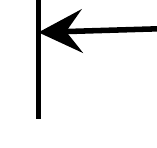
\begin{tikzpicture}
  \scalebox{5.0}{ % Adjust the 2.0 to whatever scale factor you want
    \coordinate (a) at (0,0);
    \coordinate (b) at (0,1);
    \coordinate (c) at (1,0);
    \coordinate (d) at (1,1);
    \draw (a) -- (b) node[pos=1.1,scale=0.25]{Client} (c) -- (d) node[pos=1.1,scale=0.25]{Server};
    \draw[-stealth] ($(a)!0.85!(b)$) -- node[above,scale=0.25,midway]{e} ($(c)!0.82!(d)$);
    \draw[stealth-] ($(a)!0.62!(b)$) -- node[above,scale=0.25,midway]{ekem, s} ($(c)!0.65!(d)$);
    \draw[-stealth] ($(a)!0.45!(b)$) -- node[above,scale=0.25,midway]{skem, s} ($(c)!0.42!(d)$);
    \draw[stealth-] ($(a)!0.22!(b)$) -- node[above,scale=0.25,midway]{skem} ($(c)!0.25!(d)$);
  }
\end{tikzpicture}
\caption{pqXX sequence}
\end{figure}

\vspace{.5cm}

\begin{enumerate}
    \item Client sends there ephemeral public key (e).
    \item Server sends it's static public key (s), encrypted with the KEM ciphertext (ekem) keyed to client's public ephemeral key.
    \item Client sends their static public key (s) encapsulated via KEM ciphertext (skem) keyed to server's static public key.
    \item Server sends a KEM ciphertext (skem) encapsulated using the client's static public key.
\end{enumerate}\bigskip

\vspace{1cm}

\paragraph{future improvement, option 1:}Remove the "retrieve message" command which client's use to poll for new messages. Instead the client - server Noise protocol should be designed such that clients periodically receive messages from the server without requesting or polling for them. If no message is present in the message queue on the server then the server will send the client a decoy message.

\paragraph{future improvement, option 2:}Replace the "retrieve message" command with a "send and retrieve" command whereby everytime the client sends a message they also receive a message. As per usual, perhaps some of the messages send and received are decoy messages.


\pagebreak
 
\section{Classical Sphinx and Post Quantum Sphinx}

The original Sphinx paper \citeA{sphinx} introduces the Sphinx nested encrypted packet format
using a NIKE \footnote{NIKE: non-interactive key exchange}. NIKE Sphinx can be a hybrid post quantum construction simply by using a hybrid NIKE.
Our Sphinx implementation also can optionally use a KEM \footnote{KEM: key encapsulation mechanism} instead of a NIKE, however the trade-off is that
the packet's header will take up a lot of overhead because it must store a KEM ciphertext for each hop.
Katzenpost has a completely configurable Sphinx geometry which allows for any KEM or NIKE to be used.

The Sphinx cryptographic packet format also uses these additional cryptographic primitives, the current Katzenpost
selection is: \\

\begin{itemize}
\item stream cipher: CTR-AES256
\item MAC: HMAC-SHA256
\item KDF: HKDF-SHA256
\item SPRP: AEZv5
\end{itemize}

\vspace{.5cm}

In Katzenpost the dirauths select the Sphinx geometry, each dirauth must agree with the other dirauths.
They publish the hash of the Sphinx Geometry in the PKI document so that the rest of the network entities
can validate their Sphinx Geometry. At the time of writing the namenlos network still uses classical
Sphinx with the following geometry:

\begin{figure}[ht!]
[SphinxGeometry]\\
PacketLength = 3082\\
NrHops = 5\\
HeaderLength = 476\\
RoutingInfoLength = 410\\
PerHopRoutingInfoLength = 82\\
SURBLength = 572\\
SphinxPlaintextHeaderLength = 2\\
PayloadTagLength = 32\\
ForwardPayloadLength = 2574\\
UserForwardPayloadLength = 2000\\
NextNodeHopLength = 65\\
SPRPKeyMaterialLength = 64\\
NIKEName = "x25519"\\
KEMName = ""\\
\end{figure}

In the Katzenpost implementation of Sphinx, we MAC an unencrypted two byte region at the beginning
of the Sphinx packet; This additional data region is to be used to match Sphinx version numbers.

\pagebreak

\section{Mixnet Attack Trees}

\begin{figure}[ht!]
\centering
\begin{outline}[enumerate]
   \1 Compromise Mix Node
      \2 physical Access
      \2 compromise human operator
         \3 social engineering
         \3 threat of violence
         \3 blackmail
         \3 large money bribe
         \3 legal action
         \3 police action
         \3 military action
      \2 compromise software
         \3 remote code execution vulnerability
         \3 compromise software upgrade pipeline
         \3 malware
            \4 USB stick mail interdiction
            \4 evil maid attack
\end{outline}
\caption{attacker's goal is to compromise a mix node}
\end{figure}

The above attack tree consists of all OR nodes because each of the leaves are alternative ways to achieve the sub-goal expressed by their branch
which in turn, each branch, e.g. physical access, compromise human operator, compromise software are each alternatives to the overall goal of compromising
the mix node.





\pagebreak

\citeA{int},\citeA{bayes},\citeA{n-1},\citeA{ep1}, \citeA{timing},\citeA{shor},\citeA{compulsion}

\bibliographystyleA{unsrt}
\bibliographyA{citations}

\end{document}
